%% General definitions
\documentclass{article} %% Determines the general format.
\usepackage{a4wide} %% paper size: A4.
\usepackage[utf8]{inputenc} %% This file is written in UTF-8.
%% Some editors on Windows cannot save files in UTF-8.
%% If there is a problem with special characters not showing up
%% correctly, try switching "utf8" to "latin1" (ISO 8859-1).
\usepackage[T1]{fontenc} %% Format of hte resulting PDF file.
\usepackage{fancyhdr} %% Package to create a header on each page.
\usepackage{lastpage} %% Used for "Page X of Y" in the header.
											%% For this to work, you have to call pdflatex twice.
\usepackage{enumerate} %% Used to change the style of enumerations (see below).

\usepackage{amssymb} %% Definitions for math symbols.
\usepackage{amsmath} %% Definitions for math symbols.
\usepackage{amsthm}
\usepackage{braket}
\usepackage{graphicx}
\usepackage{float}

\usepackage{tikz}  %% Pagacke to create graphics (graphs, automata, etc.)
\usetikzlibrary{automata} %% Tikz library to draw automata
\usetikzlibrary{arrows}   %% Tikz library for nicer arrow heads


%% Left side of header
\lhead{\course\\\semester\\Exercise \homeworkNumber}
%% Right side of header
\rhead{\authorname\\Page \thepage\ of \pageref{LastPage}}
%% Height of header
\usepackage[headheight=36pt]{geometry}
%% Page style that uses the header
\pagestyle{fancy}

\newcommand{\authorname}{Nico Bachmann\\Ruben Hutter}
\newcommand{\semester}{Spring semester 2023}
\newcommand{\course}{Theory of Computer Science}
\newcommand{\homeworkNumber}{4}


\begin{document}

\section*{Exercise \homeworkNumber.1}
\begin{enumerate}[(a)]
	\item
	\renewcommand{\arraystretch}{1.25}
	\begin{tabular}{ c | c }
	$w \in L$ & $w \notin L$\\
	\hline
	$0011$ & $0$\\
	$1001$ & $10$
	\end{tabular}
	
	\item
	\begin{tabular}{ c | c }
	$w \in L$ & $w \notin L$\\
	\hline
	$110$ & $111$\\
	$001$ & $0$
	\end{tabular}
	
	\item
	\begin{tabular}{ c | c }
	$w \in L$ & $w \notin L$\\
	\hline
	$0001$ & $1$\\
	$0011$ & $10$
	\end{tabular}
	
	\item
	\begin{tabular}{ c | c }
	$w \in L$ & $w \notin L$\\
	\hline
	$\emptyset$ & $1$\\
	$0$ & $10$
	\end{tabular}
	
\end{enumerate}


\section*{Exercise \homeworkNumber.2}
The language $L$ is defined by the regular expression: $(b^*ab^*ab^*)^*|b^*$

\section*{Exercise \homeworkNumber.3}
\begin{figure}[H]
		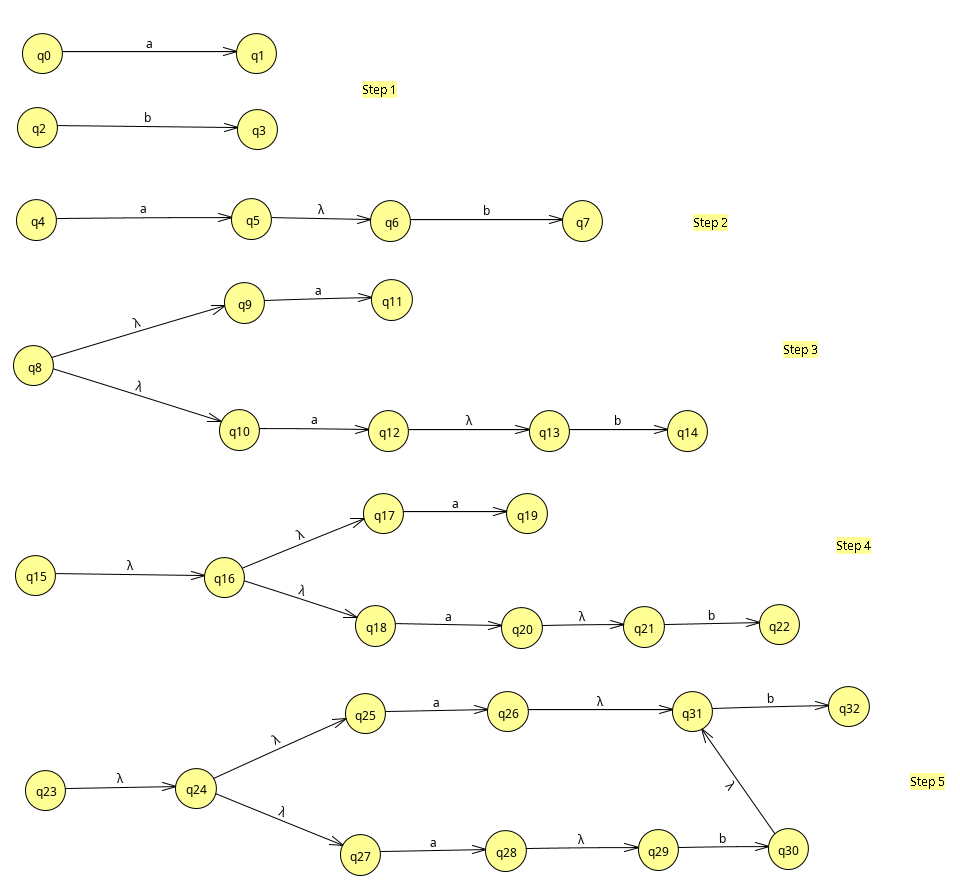
\includegraphics[width=\linewidth]{ex4.png}
		\centering
		\caption{NFA for the regular expression $\gamma = (a|ab)^*b$}
\end{figure}

\clearpage

\section*{Exercise \homeworkNumber.4}
\begin{enumerate}[(a)]
	\item
	\begin{proof}
	The language $L = \set{a^nb^mc^{n+m} \mid n, m \in \mathbb{N}_0}$ is not regular.\\
	Assume $L$ is regular. Then let $p$ be a pumping number for $L$.\\
	The word $x = a^pb^{2p}c^{p+2p}$ is in $L$ and has length $\ge p$.\\
	Let $x = uvw$ be a split with the properties of the pumping lemma.\\
	Then the word $x' = uv^2w$ is also in $L$. Since $|uv| \le p$, $uv$ consists only of symbols $a$
	and $x' = a^{p+|v|}b^{2p}c^{p+2p}$.\\
	Since $|v| \ge 1$ it follows that $(p + |v|) + 2p \neq p + 2p$ and thus $x' \notin L$.\\\\
	\textbf{Example:}\\
	$u = a^i \qquad \qquad \qquad v = a^j \qquad \qquad \qquad w = a^{n-i-j}b^mc^{n+m}$\\
	$v = v^2 \rightarrow v^2 = a^{2j}$\\
	The word is then: $x = uvvw$\\
	$uvvw = a^ia^{2j}a^{n-i-j}b^mc^{n+m} = a^{j+n}b^mc^{n+m}$\\
	$n = 2 \qquad m = 3 \qquad j = 4 \qquad \qquad \rightarrow \qquad \qquad x = aaaaaabbbccccc$\\
	\end{proof}

\end{enumerate}

\end{document}
